\chapter{NMR Data Analysis is Irreproducible}

\section{Time-domain Data Collection}
 - decaying sinusoids
 - uniform sampling
 - nyquist theorem
 - resolution
 - sweep width
 - non-uniform sampling
   - sample schedule
 - artifacts
 - pulse sequences
 - signal-to-noise


\section{Spectral processing}

The raw data collected from an NMR spectrometer is referred to as 
time-domain data.  In a typical NMR experiment, these data represent the 
sum of multiple decaying sinusoids.  These FIDs are converted to 
frequency-domain spectra which are used in further analysis.  The goal of 
this phase is to construct a frequency spectrum which indicates the resonance 
frequencies of the atoms that were observed in the experiment.  A common tool 
for such a transformation is the Fourier Transform, which is able to convert 
a data set consisting of multiple signals to a frequency spectrum.  
An example of an NMR spectrum of N-H groups is shown in Figure-\ref{nhsqc}.
Due to relaxation decreasing the amplitude of an NMR signal over time, peaks 
have an intrinsic linewidth in the frequency spectrum.

Considerations include minimization of processing artifacts, signal-to-noise 
ratio, accounting for water lines, avoiding rolling baselines and baseline 
offsets, linewidth and shape, phasing, and apodization.  Multiple software 
packages exist for carrying out this conversion \cite{nmrpipe, rnmrtk}.
These packages include functions for processing the data in specific ways to 
guarantee desirable qualities.  A typical procedure for spectral processing 
involves the sequential application of multiple functions from one of these 
packages.  At each stage, the input is a data set and associated metadata, 
which includes information such as spectral width, dwell time, and number of 
points.  Each function may require the setting of one or more parameters in 
order to proceed.  Thus, in addition to the final frequency-domain spectrum, 
the process to create generates several intermediate data sets, several 
intermediate metadata sets, and the sequence of functions used along with 
their parameterizations.  Previous work from our lab has enabled the 
convenient collection of necessary metadata during spectral 
processing \cite{connjur-wb}.


\section{Peak picking}

The Fourier Transform of a decaying sinusoid produces a frequency-domain 
spectrum with a peak at a frequency matching the oscillation frequency of 
the sinusoid.  Since NMR time-domain data consists of multiple decaying 
sinusoids caused by atoms resonating at characteristic chemical shifts, 
the frequency domain spectrum will contain peaks for every oscillating 
sinusoid present in the time-domain data.  
Peak picking involves identification of the peaks, including their
chemical shift frequencies, shape, intensity, and width.  

In general, a peak is a local maximum in the frequency spectrum.  However,
not all local maxima are necessarily peaks due to noise and artifacts.
Nor do all peaks show up as local maxima if they are weak and close to the noise
level, which causes them 
to be nearly indistinguishable from the noise and baseline; this may be due to 
sample instability such as aggregation or precipitation, or low sample 
concentration \cite{picky, munin, korzhnev2001munin, apart, autopsy, pine}
\cite{williamson2009automated, guntert2009automated, altieri2004automation,
baran2004automated}.
Since peaks have non-zero widths, peaks that are closer than their
widths will overlap, distorting measurement of their attributes and possibly
also leading to disappearance of a local maximum.  These issues complicate peak 
picking, the goal of which is to find all true signal peaks and only true 
signal peaks.
Figure-\ref{nhsqc_peaks} shows a portion of a peak-picked
NHSQC spectrum; note the overlap between some peaks, and that some -- but not
all -- low-intensity spectral features have been identified as peaks.

Given these inherent issues, a general strategy for peak picking is 
described in \cite{autopsy, picky}.
First, the noise level is estimated and points below the noise are discarded.
Next, of the remaining spectral regions, isolated areas are picked as peaks.
Finally, overlap is resolved by lineshape matching and the peaks are picked
and their attributes measured.  An optional additional step is filtering
based on symmetry and linewidth \cite{autopsy, picky}.

Correct peaks are important because they form the basis for the construction 
of GSSs, the assignment of chemical shifts to atoms, and the interpretation of 
NOESY spectra which give rise to distance restraints as a preliminary to 
structure calculation \cite{guerry2011automated}.  
Incorrect peak identification or position can result 
in misinterpretation of NOESY spectra, which could lead to false distance 
restraints between atoms which are in fact very far apart in the actual 
protein structure.

Estimates of the amount of false positive and false negative peaks picked 
by computational tools range from very low (10-40\%) to very high (70-135\%) 
\cite{pine}. 
The quality of the results generally depends on characteristics of the 
spectrum, especially the signal/noise ratio, and resolution, as well as 
characteristics of the molecule including T\textsubscript{2} (which has an 
effect on peak width) and number of atoms -- the issue being that more atoms 
means more peaks, which means a higher chance of overlap.

Since none of these approaches yields perfect 
results \cite{guerry2011automated}, manual intervention during peak picking 
is important for obtaining results of sufficiently high quality
\cite{guntert2009automated}; many peak picking 
programs allow and encourage semi-automated interaction in order to clear 
up troublesome spectral features.  
Manual intervention is often accomplished based on knowledge outside of the 
spectrum: existence, position, and shape of peaks in other spectra, knowledge 
of the solvent, characteristic artifactual patterns caused by a specific 
processing scheme, knowledge of the local dynamics of a small region of the 
protein.  \cite{williamson2009automated, guntert2009automated, 
altieri2004automation, baran2004automated}
Because of this, peak picking can often not be completely finished until 
later analysis has been accomplished.


\section{GSSs and resonances}

GSSs \cite{saga, ezassign, pistachio, autoassign1997, autoassign2001}
and resonances \cite{ccpn} are parallel to residues and atoms.
They are key to data analysis because they are the link between what is 
observed in NMR experiments and the molecular details of the sample.
Although these concepts had been used to a limited extent by earlier programs
\cite{xeasy, sparky}, more recent work has treated GSSs and resonances as 
explicit, first-class members of data analysis \cite{ccpn, bmrb}.

\subsection{Resonances}
A resonance is an NMR-visible signal which corresponds to an atom \cite{ccpn}.
In general, an atom resonates at a single characteristic frequency based
on its local environment;  the same resonance will be found at the same 
frequency across multiple experiments.  This phenomenon is used to aid in 
identification, although it is confounded by degeneracy as well as proteins
with multiple conformations.

\subsection{GSSs}
A GSS is an NMR-visible group of peaks, typically across multiple spectra,
which corresponds to a group of covalently bonded resonances; it is similar
to a residue.  
The key to GSSs is a battery of multi-dimensional pulse 
sequences designed to correlate resonances within GSSs 
\cite{cavanagh1995protein, hncacb, hnco, cbcaconh}.  These experiments are all
based on an N-H group (due to its sensitivity and chemical shift dispersion)
and correlate additional nearby nuclei through covalent bonds.

These pulse sequences use several types of overlap.  First, each pulse sequence
includes the N-H group.  Second, due to the similar scalar couplings between
N and the CA and CA(i-1) nuclei, it is possible to simultaneously correlate an
N-H group with both nearby CA nuclei; this means that each CA may be correlated
with two N-H groups, or in other words, may be a part of two GSSs. 
Third, due to the scalar coupling between N and CO(i-1), correlations to 
C*(i-1) appear in two pulse sequences of a pair (e.g. HNCACB and CBCA(CO)NH), 
while C* appear in only the HNCACB.  See Figure-\ref{ccpn_nhsqc}, 
Figure-\ref{ccpn_hncacb}, Figure-\ref{ccpn_cbcaconh}, Figure-\ref{ccpn_hnco}, 
Figure-\ref{ccpn_hncaco} for an illustration of the correlated nuclei.

These characteristics lead to a natural definition of a GSS: a root 
resonance or resonances, typically an amide H-N group, and additional 
covalently-bonded resonances.  The precise extent of a GSS is in principle 
determined by the available NMR experiments \cite{hncacb, hnco, cbcaconh}.  
In practice, a backbone GSS often is initially 
comprised of a backbone H-N, CO, CA, CB, CO(i-1), CA(i-1), and CB(i-1).  


\section{GSS and resonance construction}

This H-N matching enables grouping of peaks into GSSs; given multiple spectra
which include N-H dimensions, peaks with matching N and H chemical shifts are
determined to belong to the same GSS.
Table-\ref{pulse_sequences} shows that H-N chemical shifts are captured in 
multiple spectra, and sometimes multiple times within a single spectrum.
At a later stage, GSSs are often augmented with additional sidechain resonances.
	
In addition to GSSs of backbone resonances, H-N-rooted GSSs typically are 
visible for Asparagine and Glutamine sidechains, and smaller GSSs of 
Tryptophan sidechains are visible.  Arginine sidechains may also give rise 
to an H-N-rooted GSS under certain experimental conditions. 

The difficulty in constructing these GSSs correctly and unambiguously stems 
from the issues inherent in NMR data.  First, the success of the standard 
suite of experiments rooted in H-N -- NHSQC, HNCO, HNCACB, etc. -- depends 
on \cite{autoassign1997}: % page 600 -- `reliability`
\begin{enumerate}
  \item good dispersion, i.e. no overlap, otherwise it is difficult to determine 
    which peaks belong with which H-N-rooted spin system.
  \item the H-N chemical shifts being nearly identical across all spectra.  
    This may not be the case if there are variations in the sample or the 
    temperature.  The Block-Siegert shift and experimental error also can have 
    an effect on chemical shift.
  \item nuclei appearing at a single chemical shift.  If there are multiple 
    conformations or chemical heterogeneity \cite{autoassign1997}, 
    a nucleus may appear at multiple chemical shifts and appear to be two 
    different resonances.
  \item the presence of an H-N group -- Proline is a notable exception, and 
    so it does not show up in experiments which rely on the presence of an H-N group
  \item extraneous peaks which do not seem to fit into a spin system, or 
    peaks which do not seem to match peaks in other spectra
  \item accurate (or at least consistent) spectral referencing.  
    Misreferenced spectra will cause the same nucleus to show up at different 
    chemical shifts across multiple spectra.
  \item quality of peak-picking \cite{autoassign1997, mars}: 
    chemical shifts, lineshapes, as well as the numbers of 
    false positives, false negatives, extraneous peaks
\end{enumerate}

Computational approaches for GSS construction tend to require manual 
assistance in some cases \cite{autoassign1997, mars}.  Incorrect or 
incomplete GSSs will have negative effects on the quality of later 
analysis; several assignment tools assume that manual intervention will 
verify and, if necessary, correct the GSSs \cite{williamson2009automated}; 
this allows the tools to be conservative in their 
predictions \cite{autoassign1997}.  However, it may not be 
possible to unambiguously and completely construct GSSs until the results 
of later analysis are available: some approaches use NOESY peaks and 
assignments as well as structure results to verify and correct GSSs 
\cite{autoassign1997}.

Figure-\ref{nhsqc_hncacb} shows an example of matching peaks between two
spectra.  The quality of the match -- how closely the chemical shifts line up,
as well as the lack of overlapping peaks -- means the peaks are easily
identified as members of the same GSS.


\section{Backbone spin systems and resonances: typing and sequence-specific assignment}

Once GSSs have been constructed, analysis continues with four simultaneous 
assignment subtasks: resonance typing, GSS typing, GSS to
GSS sequentially, and GSS to specific residues of the sample of interest.

\subsection{Assignment of resonance to atomtype}

Before assigning a resonance to a specific 
atom, the atomtype of a resonance may be assigned.  In an HNCO experiment, 
this is typically straightforward, because for each backbone spin system, 
the H dimension always corresponds to the backbone H, the N dimension always 
corresponds to the backbone N, and the C dimension always corresponds to the 
backbone C(i-1).  However, the situation is more complicated in an HNCACB 
experiment, as there are generally four choices of atomtype assignment for 
the C dimension:  CA, CB, CA(i-1), and CB(i-1).  Thus, the resonance given 
by the C dimension of each peak must be assigned one of these choices.  
Reasons for choosing a specific assignment include peak sign, as well as 
chemical shift compared to statistics available in the BMRB.  In addition, 
the overlap between experiment pairs such as the HNCACB and CBCA(CO)NH 
facilitates resonance-atomtype assignment: while the CA(i-1) and CB(i-1) 
are expected to appear in both experiments at the same chemical shift for 
a given backbone H-N root, the CA and CB are expected to appear only in the 
HNCACB spectrum.

\subsection{Assignment of amino acid type to GSS}

Correspondingly, GSSs are also assigned amino acid types.  This phase 
interacts strongly with the assignment of atomtypes to resonances, in 
that the possible atomtypes to which a resonance may be assigned depends 
on the amino acid type, and the expected chemical shift ranges for various 
atomtypes depends on amino acid type as well.  For instance, GSSs assigned 
to the Glycine amino acid type should not have a CB; and the CB resonance's 
chemical shift of a GSS assigned to Alanine is expected to be very different 
from all other CB chemical shifts.  Backbone amino acid types may be split 
into several categories \cite{saga} based on BMRB statistics for 
CA and CB chemical shifts \cite{bmrb}:
\begin{enumerate}
  \item Ala
  \item Gly 
  \item Pro
  \item Ser, Thr
  \item Val, Met, Lys, His, Arg, Glu, Gln, Trp, Cys
  \item Asp, Asn, Ile, Leu, Phe, Tyr
\end{enumerate}
However, GSS typings are complicated by several factors.  First, GSS typing 
requires correct and complete GSS construction.  Second, correctly assembled 
GSSs may include overlapped or extraneous peaks, expected peaks (based on a 
spectrum's typical results) may also be missing.  Third, most GSSs can not 
be uniquely typed based solely on CA and CB chemical shifts, as groups 5 and 
6 (above) as well as 4 are ambiguous.  Fourth, sidechain GSSs must be 
identified and separated.

\subsection{Assignment of GSS to GSS sequentially}

Sequential GSS assignments exploit the previously mentioned overlap of pulse
sequences such as the HNCACB and HN(CA)CO.  Sequential GSSs 
are expected to have CA/CA(i-1), CB/CB(i-1), and CO/CO(i-1) resonances at 
identical chemical shifts.  This duplication enables sequential assignment 
of GSSs.  Note that there is substantial interaction between atomtype-resonance 
assignment and sequential GSS assignment: assigning two GSSs sequentially 
implies the CB vs CB(i-1), CA vs CA(i-1), and C vs C(i-1) atomtype assignments 
of the resonances in both GSSs; knowing the atomtype-resonance assignments of 
two spin systems can prevent their sequential assignment (if, for example, the 
matching resonances are both CB(i-1)); and not knowing the atomtype-resonance 
assignment implies that the sequential GSS assignment may be invalid.  
Sequential GSS assignment is complicated by: 
\begin{enumerate}
  \item missing peaks, possibly caused 
  by local dynamics, which reduce the number of overlapping resonances between 
  potential sequential GSSs, and can also disrupt atomtype assignments of 
  resonances; 
  \item extraneous peaks, which may be false positives or caused by 
  multiple conformations of the protein, causing incorrect matches
  \item degeneracy of chemical shifts:  given two GSSs with identical CA(i-1) 
  and CB(i-1) resonances, as well as a third GSS with matching CA and CB 
  resonances, it is impossible to unambiguously assign sequentially solely 
  on the basis of chemical shift matching between the two GSSs 
  \cite{autoassign1997}.
\end{enumerate}

An example of GSS overlap is shown in Figure-\ref{hncacb_overlap}.  Green peaks
are CA, and purple peaks are CB; note that one each of green and purple peaks
match between the two GSSs.

\subsection{Assignment of GSS to specific residue of sample of interest}

The final piece of backbone analysis is assignment of GSSs to specific 
residues.  Since backbone GSSs are H-N-rooted, a GSS is assigned to a 
backbone-amide; this implies the assignment of resonances to atoms as well, 
based on matching of atomtypes.  When a typical GSS is assigned to a residue, 
the H, N, C, C(i-1), CA, CA(i-1), CB, and CB(i-1) atoms will be assigned 
resonances as well.  Sequence-specific assignment interacts heavily with 
sequential GSS assignment, because the protein sequence must be compatible 
with the GSS sequence, where `compatible' means that the amino acid types 
of the GSS match those of the protein sequence.  Note that full assignment 
of amino acid type to GSS is not a prerequisite for GSS-residue assignment; 
in fact, GSS-residue assignment may lead to GSS-amino acid type assignment 
for sequentially connected GSSs.  GSS-residue assignment is facilitated by 
long chains of sequential GSSs in which some of the GSSs are typed as Serine, 
Threonine, Glycine, or Alanine.  The longer a GSS chain, the fewer places it 
might possibly fit into the protein sequence \cite{saga}.  Also, 
as sequence-specific assignment proceeds, the number of unassigned GSSs and 
residues decreases; the result is that initially ambiguous assignments become 
unambiguous as choices are removed.  Conversely, complications arise from 
incomplete sequential GSS assignments resulting in short, ambiguous chains.  
The presence of prolines generally ends chains due to the lack of a backbone 
H-N group.  Missing GSSs also terminate chains.  Relatively few Ser, Thr, Gly, 
and Ala residues means the number of unambiguous anchor points will be lower.

Figure-\ref{ss-residue} shows an example of sequence-specific GSS assignment.
Although not all of the GSSs have been typed, the presence of a Glycine and
Serine in the GSS chain reduces the possible assignments to residues.
Additionally, the length of the GSS chain helps reduce the ambiguity compared
to shorter GSS chains.


\section{Sidechain: spin system and resonance assignment}

The next group of experiments collects chemical shifts of sidechain atoms.  
These experiments include 
the HBHA(CO)NH \cite{hbhaconh} in Figure-\ref{ccpn_hbhaconh}, 
the C(CO)NH-Tocsy \cite{cconhtocsy} in Figure-\ref{ccpn_cconhtocsy}, 
the HC(CO)NH-Tocsy \cite{hcconhtocsy} in Figure-\ref{ccpn_hcconhtocsy}, 
the HCCH-Tocsy \cite{hcchtocsy} in Figure-\ref{ccpn_hcchtocsy}, 
and aromatic Tocsys.  The purpose of these experiments is to 
obtain the chemical shift values of sidechain resonances of protons, since 
proton frequencies are necessary in order to interpret NOESY spectra.  To 
interpret these spectra, the peaks must be assigned to GSSs and atomtypes 
must be assigned to the new resonances. While several of these experiments 
are also rooted in backbone H-N groups, facilitating the addition of peaks 
to the correct GSS, others -- such as the HCCH-Tocsy -- are not.  These are 
analyzed by the matching of resonance chemical shifts with those from other 
experiments targeting sidechains.  Atomtype-resonance assignments can generally 
be made with reference to compiled BMRB statistics.  Complications in this 
phase include: stereospecificity -- nuclei such as HA2 and HA3 may give rise 
to different chemical shifts, but resolving the correspondence may be 
impossible without further data; overlap -- especially in the HCCH-Tocsy 
where sidechains of the same amino acid type but different residue may have 
many closing matching chemical shifts; overlap between resonances within the 
same GSS, especially in Leu and Ile; missing and extraneous data; and the 
difficulty of both obtaining and unambiguously interpreting aromatic data.  
New approaches for sidechain data collection and assignment have recently 
been developed \cite{mobli2010non, hiller2008apsy} which seek to address 
these issues by reducing ambiguity of chemical shifts.


\section{NOESY peak-picking and assignment}

In NOESY spectra, each true peak indicates a pair of protons within 
approximately 5 Angstroms of each other.  This is different from the 
correlation spectra discussed earlier, in which peaks indicate covalently 
bonded atoms; NOESY spectra do not depend on covalent bonds but rather 
depend on spatial proximity.  Thus, each NOESY peak contains some information 
about the actual three-dimensional structure of a molecule, if it can be 
determined which protons give rise to the peak.  Analysis of NOESY spectra 
requires chemical shift assignments of atoms, and uses that information to 
determine the protons involved in a peak.  Considerations used to analyze 
NOESY spectra include: symmetry -- a peak is expected to correspond to a 
matching peak with the frequencies of the two 1H dimensions swapped; patterns 
based on known proximity of atoms from the primary sequence giving rise to 
many short-distance NOE peaks; network anchoring.  Complications include 
overlap caused by degenerate chemical shifts of protons, leading to 
ambiguous interpretations of peak assignments; this can be greatly mitigated 
by the use of an extra dimension:  15N- or 13C-edited NOESY spectra reduce 
the ambiguity, as well as incorrect or incomplete chemical shift assignments.

NOESY assignment is generally done automatically \cite{cyana2004, aria2003}.  
NOESY peak-picking may be automated as well \cite{munin, korzhnev2001munin}.


\section{Structure calculation}

Cyana is able to calculate a three-dimensional structure from NOESY peaks, 
chemical shift assignments, and distance restraints \cite{cyana2004, aria2003} 
using an iterative approach to NOESY peak assignment and building structural 
models.  It also requires secondary structure information as input, which can 
be calculated from chemical shift assignments using a program such as 
\cite{talos+}.  Chemical shift assignments may also be used to 
calculate potential structures \cite{cs-rosetta}.  Additional programs 
may be used to refine structures \cite{amber, xplor-nih}.  This phase 
generally does not require manual intervention.


\section{Discussion}

The inherent NMR issues of ambiguous, missing, and extraneous data cause 
problems throughout the entire analysis process.  Correctly dealing with 
these issues is difficult, but absolutely critical in order to obtain 
high-quality results \cite{williamson2009automated, guntert2009automated, 
altieri2004automation, baran2004automated}.  As yet, computational tools 
are not able to deal perfectly with these issues.  
Most tools have several basic limitations: 
\begin{enumerate}
  \item they require high-quality input in order to function correctly 
  \cite{saga, abacus_assignment, mars, autoassign2001, ezassign, pine, cyana2004}; 
  this input is generally assumed to have been manually prepared in order 
  to meet the stringent quality requirements of completeness and absence of 
  extraneous results
  \item even with high-quality input data, tools are not able to produce 
  perfect results 
  \item tools perform differently in different contexts, although 
  performance generally decreases as protein size increases and spectral quality 
  decreases
  \item manual verification and correction of the results is assumed, 
  even for tools that claim to be fully automated 
  \cite{williamson2009automated, guntert2009automated, altieri2004automation,
  baran2004automated}
\end{enumerate}

A key limitation of many analysis tools is that they are viewed as part of a 
pipeline: input is transformed into output, which becomes the input for the 
next stage, and so on \cite{pine}.  This may explain why these tools 
are not able to produce better results:  full analysis, including peak-picking, 
GSS construction, assignment, and so on, can make use of information from 
multiple stages.  Humans, performing manual interventions, are able to bring 
this additional information to bear to make specific interpretations; however, 
many of these tools do not.  Thus, PINE and related efforts  
are an exciting effort to loosen these artificial restrictions.  Initial 
results are promising, and show a marked improvement, although manual 
intervention is still assumed to be necessary in order to obtain the best 
results \cite{pine}.  Further tools such as \cite{shiftx2, cheshire}, 
which calculate chemical shifts from structure, provide additional means 
for bringing additional information to bear, helping to validate assignments.

Another exciting development is the rise of probabilistic methods 
\cite{saga, pine}.  These methods reflect the reality that the 
confidence of a specific interpretation depends on the exact state of the 
data; in other words, an assignment which is 50\% confident given only an 
HNCA spectrum may become 90\% confident if an HN(CO)CA spectrum is added.  
The significance of this confidence level is that it enables easy tracking 
of ambiguous and/or low-confidence interpretations -- i.e. those that stand 
to benefit from collecting additional data sets.  By including confidence 
values on all assignments, an understanding of the troublesome areas is 
facilitated.  This helps to reduce the cost of cascading errors -- if the 
uncertainty is tracked as a confidence level, further interpretations based 
on a highly uncertain datum will also receive low confidence levels.  In 
addition, confidence levels are an alternative to the inherent balance 
between completeness and correctness -- it is no longer necessary to 
sacrifice one for the other \cite{autoassign2001, pine}.


\section{Conclusions}

Manual analysis plays a critical role in NMR data analysis, due to the inherent 
issues involved in analysis and to the large amount of information which must 
be brought to bear to solve difficult cases.  Although spectral processing, 
NOESY assignment, and structure calculation have been automated, peak-picking, 
GSS construction, and assignment of both resonances and GSSs have not been 
completely automated.  Manual intervention is assumed to be necessary by 
most tools, even automated ones, to ensure the completeness and correctness 
of results.  However, despite the importance that manual intervention plays 
in analysis, the specific modifications made and their reasons for -- 
which may be quite complicated -- are not captured \cite{guntert2009automated}.  
Thus, the metadata of manual intervention is lost, and analysis is 
irreproducible.


% tables
\clearpage
\section{Tables}

\begin{table}[h] % if I don't add the [h], the table comes before the section title
    \begin{tabular}{ | c || c | c | c | c | c |}
    \hline
              & NHSQC & HNCO & HN(CA)CO & HNCACB & CBCA(CO)NH \\
    \hline
      H       & 1 & 1 & 2 & 4 & 2 \\
    \hline
      N       & 1 & 1 & 2 & 4 & 2 \\
    \hline
      CO      & 0 & 1 & 0 & 0 & 0 \\
    \hline
      CO(i-1) & 0 & 1 & 1 & 0 & 0 \\
    \hline
      CA      & 0 & 0 & 0 & 1 & 0 \\
    \hline
      CA(i-1) & 0 & 0 & 0 & 1 & 1 \\
    \hline
      CB      & 0 & 0 & 0 & 1 & 0 \\
    \hline
      CB(i-1) & 0 & 0 & 0 & 1 & 1 \\
    \hline
    \end{tabular}
    \caption{The number of times nuclei typically appear in pulse sequences}
    \label{pulse_sequences}
\end{table}


% figures
\clearpage
\section{Figures}

\begin{figure}[h]
  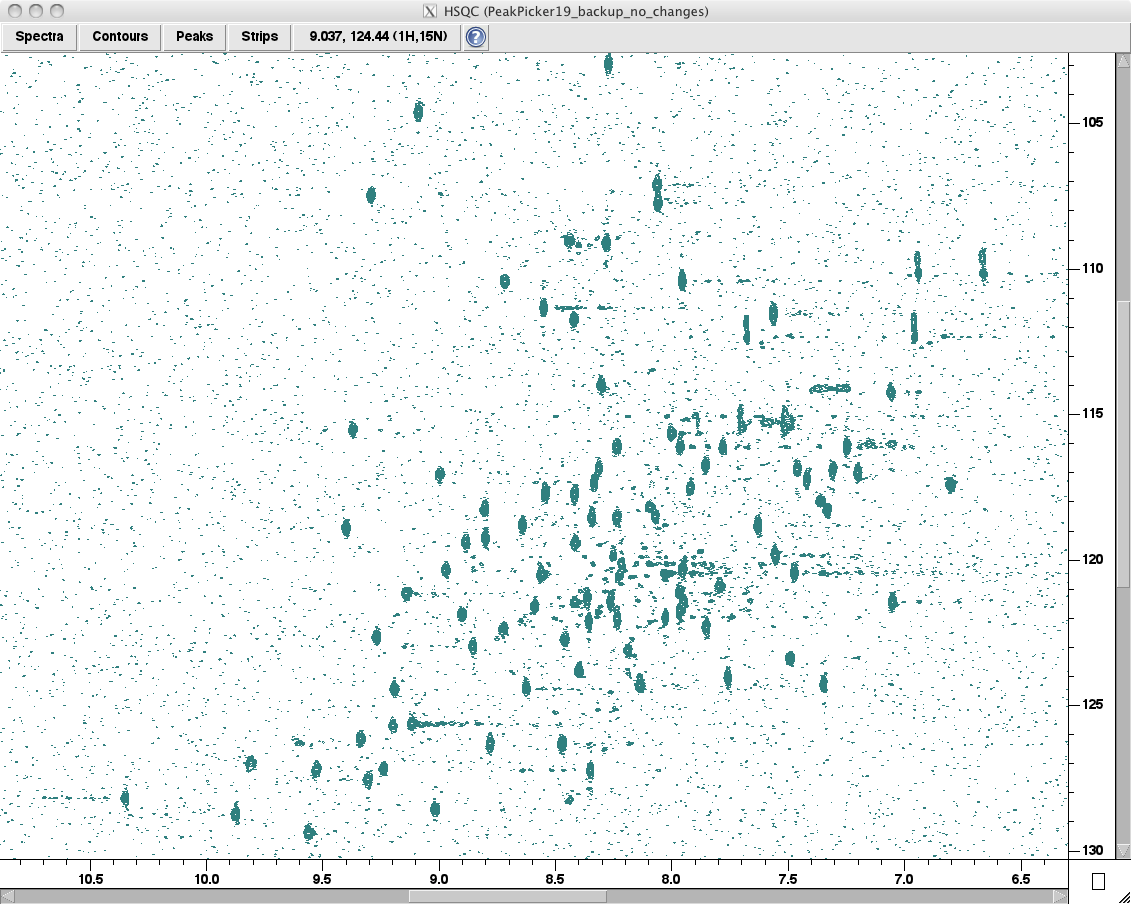
\includegraphics[scale=0.35]{figures/nhsqc}
  \caption[A frequency-domain NHSQC spectrum]
          {A frequency-domain NHSQC spectrum. 
           The x- and y-axes are nitrogen and proton, respectively.}
  \label{nhsqc}
\end{figure}

\begin{figure}
  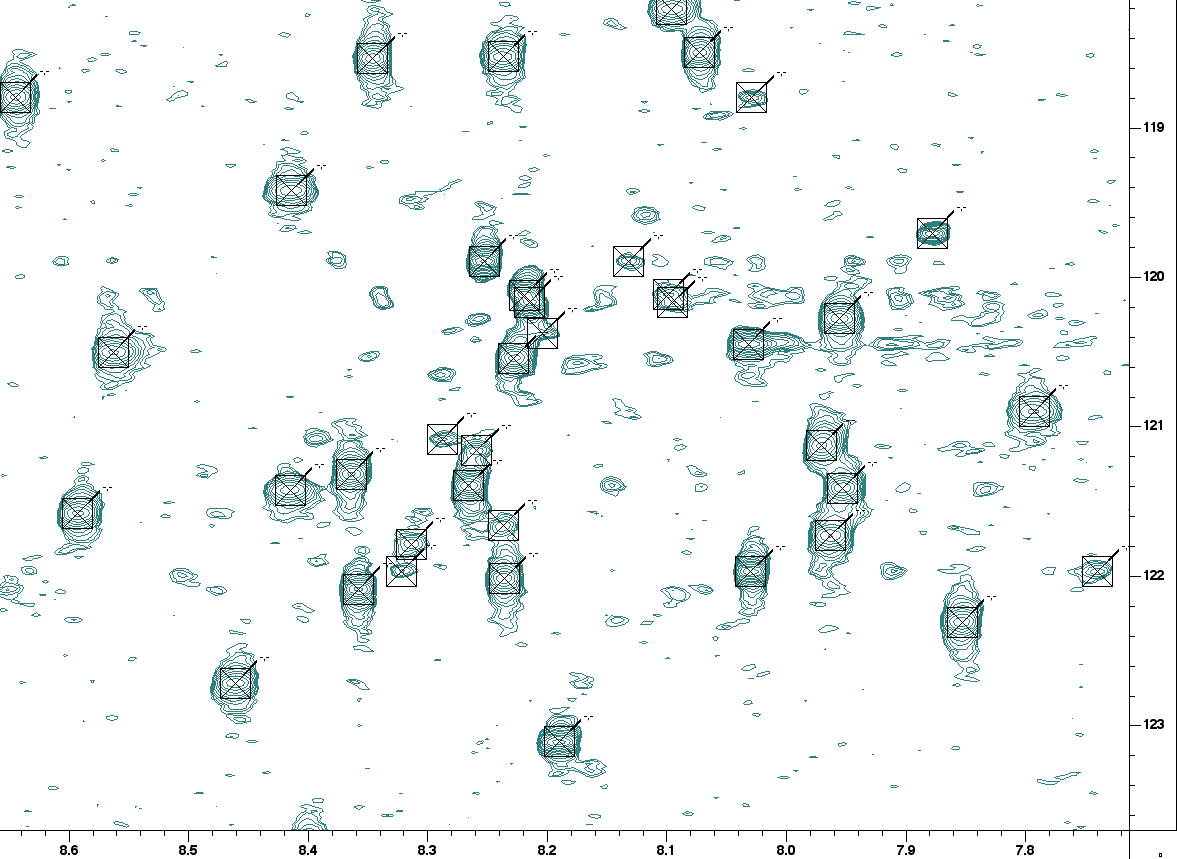
\includegraphics[scale=0.35]{figures/nhsqc_peaks}
  \caption[A peak-picked NHSQC spectrum]
          {A peak-picked NHSQC spectrum. 
           Peaks are indicated by black squares and crosses.}
  \label{nhsqc_peaks}
\end{figure}

\begin{figure}
  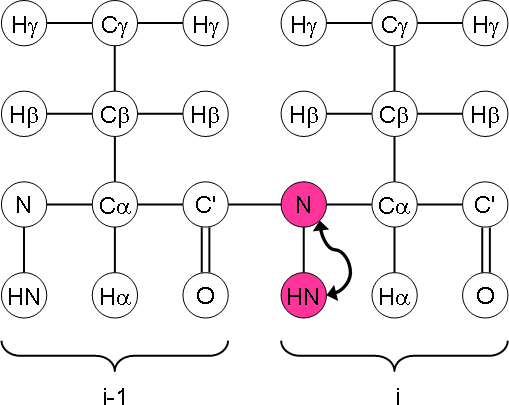
\includegraphics[scale=0.75]{figures/ccpn_nhsqc}
  \caption[The nuclei correlated by an NHSQC.]
          {The nuclei correlated (red) by an NHSQC.}
  \label{ccpn_nhsqc}
\end{figure}

\begin{figure}
  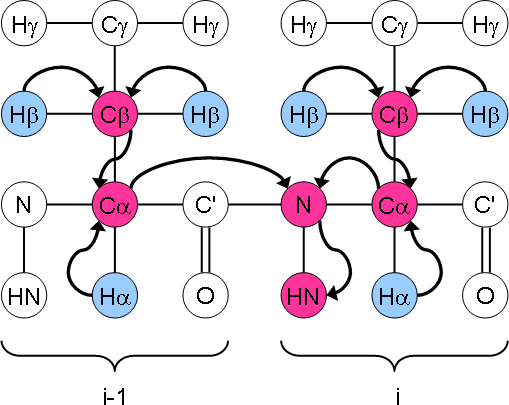
\includegraphics[scale=0.75]{figures/ccpn_hncacb}
  \caption[The nuclei correlated by an HNCACB.]
          {The nuclei correlated (red) by an HNCACB.}
  \label{ccpn_hncacb}
\end{figure}

\begin{figure}
  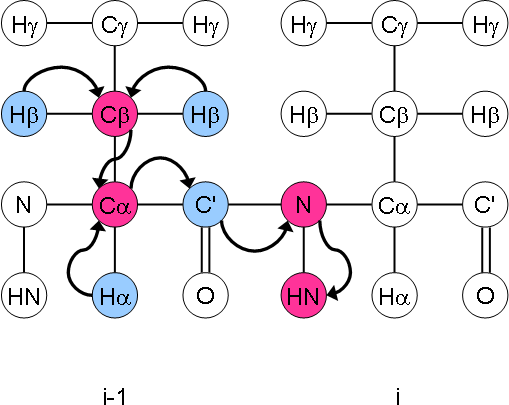
\includegraphics[scale=0.75]{figures/ccpn_cbcaconh}
  \caption[The nuclei correlated by a CBCA(CO)NH.]
          {The nuclei correlated (red) by a CBCA(CO)NH.}
  \label{ccpn_cbcaconh}
\end{figure}

\begin{figure}
  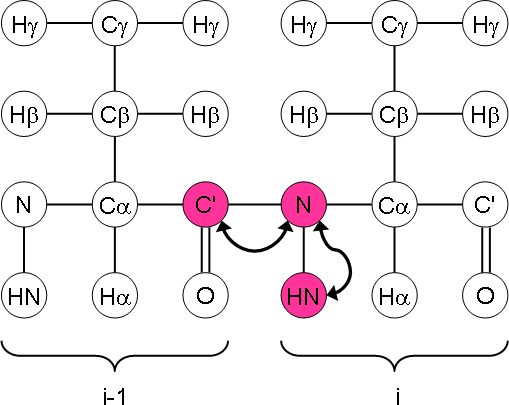
\includegraphics[scale=0.75]{figures/ccpn_hnco}
  \caption[The nuclei correlated by an HNCO.]
          {The nuclei correlated (red) by an HNCO.}
  \label{ccpn_hnco}
\end{figure}

\begin{figure}
  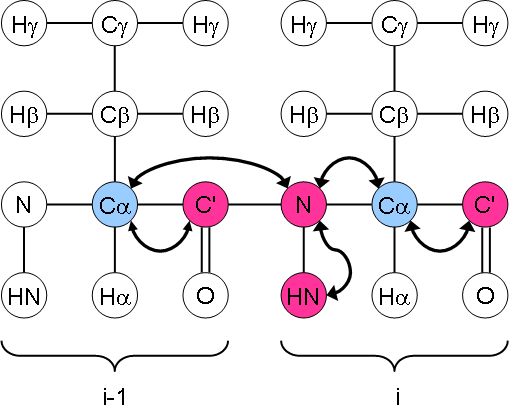
\includegraphics[scale=0.75]{figures/ccpn_hncaco}
  \caption[The nuclei correlated by an HN(CA)CO.]
          {The nuclei correlated (red) by an HN(CA)CO.}
  \label{ccpn_hncaco}
\end{figure}

\begin{figure}
  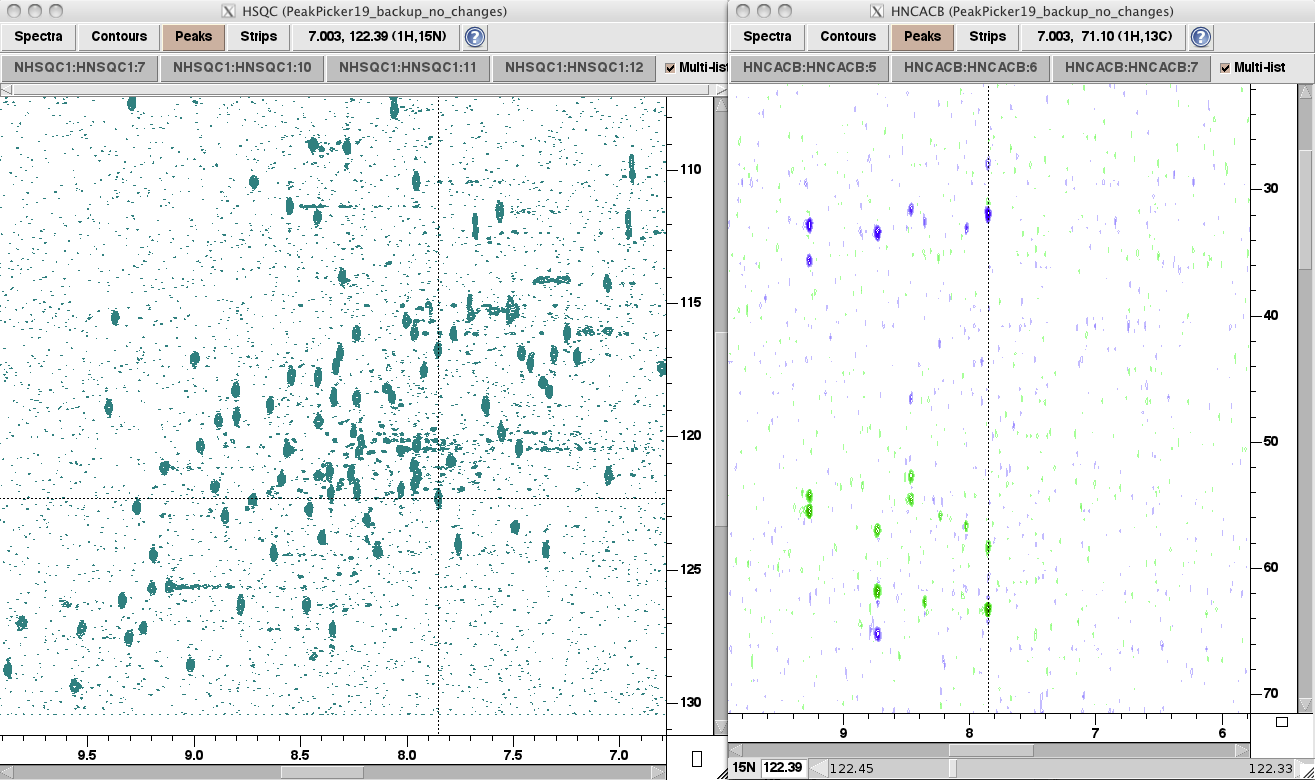
\includegraphics[scale=0.3]{figures/nhsqc_hncacb}
  \caption[Matching peaks between an NHSQC and an HNCACB spectrum]
          {Matching peaks between an NHSQC and an HNCACB spectrum.
           This likely indicates that the peaks belong to the same GSS.}
  \label{nhsqc_hncacb}
\end{figure}

\begin{figure}
  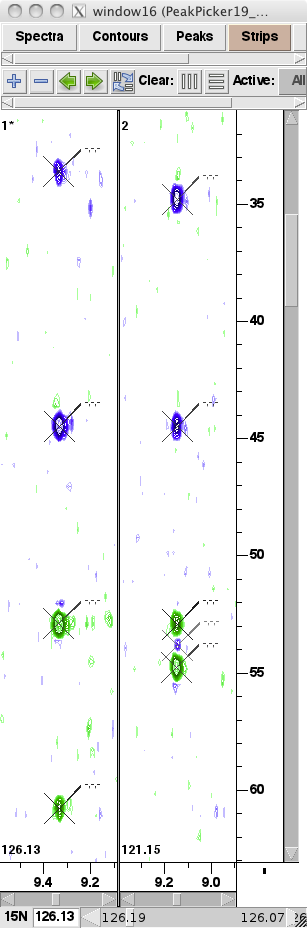
\includegraphics[scale=0.35]{figures/hncacb_overlap}
  \caption{Overlap of Carbon resonances in an HNCACB spectrum.}
  \label{hncacb_overlap}
\end{figure}

\begin{figure}
  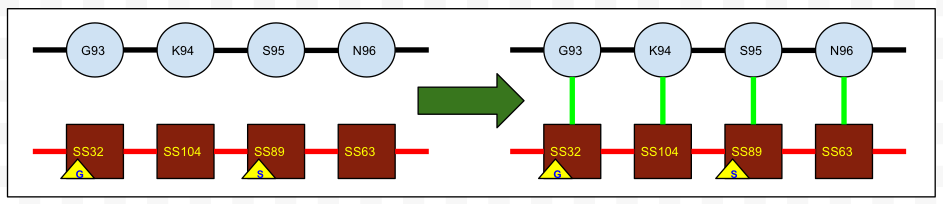
\includegraphics[scale=0.45]{figures/ss-residue}
  \caption[Assignment of a GSS chain to residues]
          {Assignment of a GSS chain to residues.  The circles are residues,
           black lines are peptide bonds, squares are GSSs, red lines are 
           sequential GSS assignments, and green lines are GSS-residue 
           assignments.}
  \label{ss-residue}
\end{figure}

\begin{figure}
  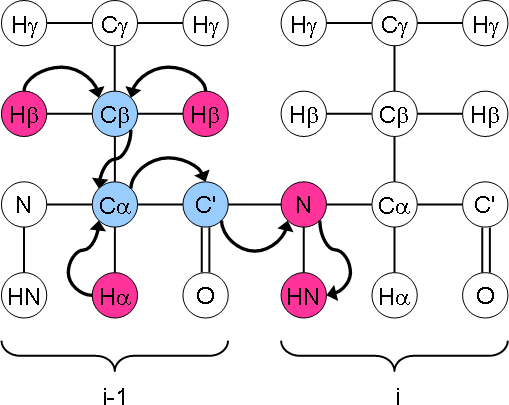
\includegraphics[scale=0.75]{figures/ccpn_hbhaconh}
  \caption[The nuclei correlated by an HBHA(CO)NH.]
          {The nuclei correlated (red) by an HBHA(CO)NH.}
  \label{ccpn_hbhaconh}
\end{figure}

\begin{figure}
  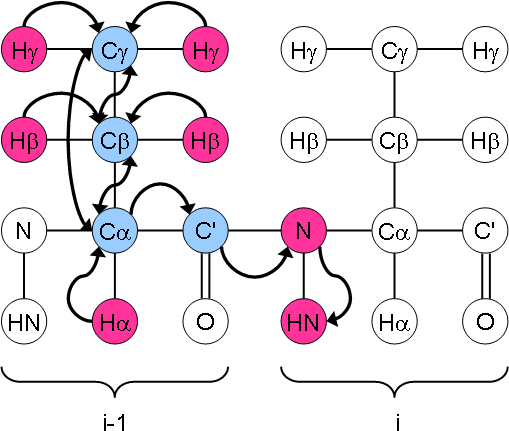
\includegraphics[scale=0.75]{figures/ccpn_hcconhtocsy}
  \caption[The nuclei correlated by an H(CCO)NH-Tocsy.]
          {The nuclei correlated (red) by an H(CCO)NH-Tocsy.}
  \label{ccpn_hcconhtocsy}
\end{figure}

\begin{figure}
  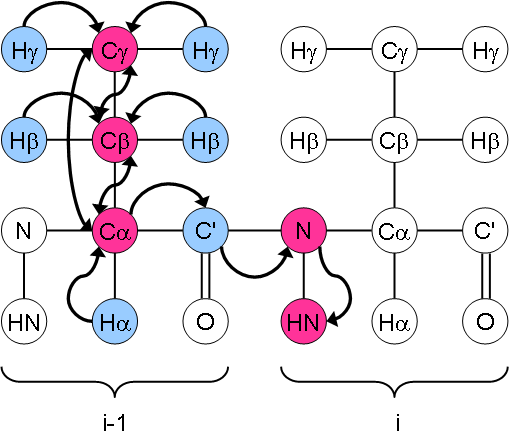
\includegraphics[scale=0.75]{figures/ccpn_cconhtocsy}
  \caption[The nuclei correlated by a C(CO)NH-Tocsy.]
          {The nuclei correlated (red) by a C(CO)NH-Tocsy.}
  \label{ccpn_cconhtocsy}
\end{figure}

\begin{figure}
  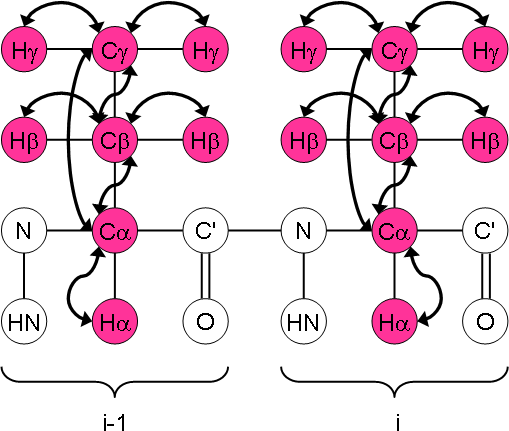
\includegraphics[scale=0.75]{figures/ccpn_hcchtocsy}
  \caption[The nuclei correlated by an HCCH-Tocsy.]
          {The nuclei correlated (red) by an HCCH-Tocsy.}
  \label{ccpn_hcchtocsy}
\end{figure}

